%%%% SEITENRAENDER, SCHRIFTGROESSE UND ZEILENABSTAND NICHT ABAENDERN => SONST GIBT ES PUNKTEABZUG
\documentclass[a4paper,11pt,singlespacing]{article}
\usepackage[left=2.5cm,right=2.5cm,top=2.5cm]{geometry}
\usepackage{setspace}
\usepackage[utf8]{inputenc}
\usepackage{graphicx}
\usepackage{color}
\usepackage{hyperref}
\usepackage{biblatex}
\usepackage{listings,xcolor}
\usepackage{pdfpages}
\usepackage{amsmath}

%for coding snippet
\definecolor{codegreen}{rgb}{0,0.6,0}
\definecolor{codegray}{rgb}{0.5,0.5,0.5}
\definecolor{codepurple}{rgb}{0.58,0,0.82}
\definecolor{backcolour}{rgb}{0.95,0.95,0.92}
\lstdefinestyle{mystyle}{
    backgroundcolor=\color{backcolour},   
    commentstyle=\color{codegreen},
    keywordstyle=\color{magenta},
    numberstyle=\tiny\color{codegray},
    stringstyle=\color{codepurple},
    basicstyle=\ttfamily\footnotesize,
    breakatwhitespace=false,         
    breaklines=true,                 
    captionpos=b,                    
    keepspaces=true,                 
    numbers=left,                    
    numbersep=5pt,                  
    showspaces=false,                
    showstringspaces=false,
    showtabs=false,                  
    tabsize=2
}

\lstset{style=mystyle}


%opening
\title{DockerSec: Cybersecurity Training and Testing Environment}
\author{
	Rémi JARDRET 20741372,
	Stéphane SIMON 21641381
	}


\begin{document}
% Absatzeinrückung verhindern
\setlength{\parindent}{0ex}


\begin{titlepage}
	
	\newcommand{\HRule}{\rule{\linewidth}{0.5mm}} % Defines a new command for the horizontal lines, change thickness here
	
	\center % Center everything on the page
	
	%----------------------------------------------------------------------------------------
	%	HEADING SECTIONS
	%----------------------------------------------------------------------------------------
		
	
	\includegraphics[width=7cm]{images/rwu_logo.png}\\[1.5cm] % Include a department/university logo - this will require the graphicx package
	
	\textsc{\LARGE University of Applied Sciences Ravensburg Weingarten}\\[1.5cm] 
	\textsc{\Large Department of
		Electrical Engineering
		and Computer Science}\\[0.5cm]
	\textsc{\large Bachelor Project}\\[0.5cm] 
	
	%----------------------------------------------------------------------------------------
	%	TITLE SECTION
	%----------------------------------------------------------------------------------------
	
	\HRule \\[0.4cm]
	{ \huge \bfseries DockerSec: Cybersecurity Training and Testing Environment}\\[0.4cm] 
	\HRule \\[3.5cm]
	
	%----------------------------------------------------------------------------------------
	%	AUTHOR SECTION
	%----------------------------------------------------------------------------------------
	
	\begin{minipage}{0.4\textwidth}
		\begin{flushleft} \large
			\emph{Author:}\\
   			Rémi \textsc{JARDRET}\\
			20741372\\
			Stéphane \textsc{SIMON}\\
			21641381
		\end{flushleft}
	\end{minipage}
	~
	\begin{minipage}{0.4\textwidth}
		\begin{flushright} \large
			\emph{Supervisor:} \\
			Herr Benjamin \textsc{Stähle}\\ % Supervisor's Name
            \& \\
			Herr Norbert \textsc{Perk} % Supervisor's Name
		\end{flushright}
	\end{minipage}\\[5cm]
	
	% If you don't want a supervisor, uncomment the two lines below and remove the section above
	%\Large \emph{Author:}\\
	%John \textsc{Smith}\\[3cm] % Your name
	
	%----------------------------------------------------------------------------------------
	%	DATE SECTION
	%----------------------------------------------------------------------------------------
	
	{\large \today}\\[5cm] % Date, change the \today to a set date if you want to be precise
	
	%----------------------------------------------------------------------------------------
	%	LOGO SECTION
	%----------------------------------------------------------------------------------------

	%----------------------------------------------------------------------------------------
	
	\vfill % Fill the rest of the page with whitespace
	
\end{titlepage}


\tableofcontents
\pagebreak



\section{Introduction}

\subsection{Motivation}
The inspiration for this project stemmed from our Linux Administration course at our home
institution. In this course, we were tasked with creating an environment comprising a minimum of six virtual machines (VMs) running different Linux distributions. However, this proved to be a labor-intensive process that demanded a lot of hardware resources.
On the other side, we also attended classes in cybersecurity, specifically pentesting, where we frequently encountered similar environments. In these classes, we often found ourselves spending around three sessions setting up the environment before we could start our training and pentesting.
Following this observation, we concluded that a pre-configured environment with optimized resource utilization would be highly beneficial. Ideally, this environment should be quick and easy to set up. Docker, and in particular Docker Compose, emerged as the perfect solution, offering a streamlined and state-of-the-art solution.            

\subsection{Problem}
From conceptualizing a pre-configured environment with optimized resource utilization to the actual implementation of the project, we encountered numerous challenges. This involved decisions regarding the tools to employ, defining our approach, and assessing whether our solution would outperform a traditional virtual machines setup. Consequently, a comparative analysis between our solution and the conventional approach is imperative to identify any potential enhancements.

\subsection{Objectives}
This project is driven by several key objectives, each addressing specific challenges and needs:

\begin{enumerate}
    \item \textbf{Streamlined Environment Setup:} One primary objective is to eliminate the time-consuming and intricate setup of environments for learning and training purposes. The current process of configuring multiple virtual machines (VMs) running different Linux distributions can be arduous, and we aim to simplify this.
    
    \item \textbf{Ease of Deployment:} We also seek to address the challenges related to setting up these environments, making it more user-friendly. The configuration of complex network topologies, including DHCP, DNS, HTTP servers, DMZs, firewalls, and routers, can be daunting for learners and security enthusiasts.
    
    \item \textbf{Resource Optimization:} Resource optimization is a crucial goal. We want to ensure that the environment we provide is efficient in terms of resource utilization, enabling users to run multiple instances simultaneously without overwhelming hardware resources.
\end{enumerate}

Taking these overarching objectives into account, we have defined three specific goals for our project:

\begin{itemize}
    \item \textbf{Facilitating System Administration Learning:} We aim to create an environment where users can explore and understand the intricacies of system administration. This involves gaining insights into the setup and configuration of different components such as "computers," networks, and services. Users can investigate, extend, and experiment with various aspects of system administration.

    \item \textbf{Enhancing Pentesting Training:} Our project seeks to provide a robust platform for pentesting training. This environment will enable users to practice various types of attacks, such as spoofing, scanning, and brute-forcing... Almost all of the Cyber Kill Chain\footnote{\url{https://www.lockheedmartin.com/en-us/capabilities/cyber/cyber-kill-chain.html}} can be experimented on this environment.

    \item \textbf{Exploring Docker Capabilities:} This project will serve as an exemplary case among many, enabling learners to delve into more complex Docker setups and explore the full extent of Docker's capabilities.

\end{itemize}

In practical terms, our project aims to deliver an environment consisting of Linux-based containers with integrated features, that will we detail in the next part. This environment will serve as a multifaceted learning platform. Users can look at the configurations, experiment with various scenarios, and advance their knowledge in both system administration and cybersecurity. With the ability to simulate attacks, the project aims to offer an arena for learning and practice.


\section{Project Requirements}\label{ProjectRequirements}

\subsection{Context}
This project has its roots in our Linux Administration course at our home institution. In this course, we were tasked with creating an environment comprising a minimum of six virtual machines (VMs) running different Linux distributions. However, this turned out to be a labor-intensive process that required a significant amount of hardware resources.\\

On the other hand, we also attended classes in cybersecurity, specifically pentesting, where we frequently encountered similar environments. In these classes, we often found ourselves spending approximately three sessions setting up the environment before we could commence our training and pentesting.\\

Following this observation, we concluded that a pre-configured environment with optimized resource utilization would be highly beneficial. Ideally, this environment should be quick and easy to set up. Docker, and particularly Docker Compose, emerged as the perfect solution, offering a streamlined and state-of-the-art approach.\\

This project is part of an Erasmus exchange program and is taking place during the Linux Administration course at the RWU. The subject matter not only holds potential value for the RWU but also for future students. As part of the Erasmus experience, we aim to create a solution that not only streamlines our coursework but can be a valuable resource for students and beyond.\par

\newpage

\subsection{Requirements}
As mentionned in our previous document called "Project Sketch", we will deploy the following infrastructure (Appendix \ref{Appendix1})

\subsubsection{Functional Requirements}
From a functional perspective, this environment is designed to provide a scalable and efficient platform for cybersecurity training and Linux administration testing. The primary objective is to achieve a noticeable reduction in host system resource utilization when compared to traditional setups using virtual machines.\\

In addition to energy efficiency, this environment should be readily operational with a simple "docker compose" command, emphasizing ease of deployment. Rigorous testing is essential to identify and address potential system-specific issues, ensuring seamless functionality. The initial focus is on enabling deployment on Unix host systems, with a secondary objective to extend compatibility to Windows host systems.\\

Furthermore, this project aims to be a valuable learning resource. Both pentesters and Linux administrators should be able to acquire knowledge through this environment. This necessitates the inclusion of diverse scenarios, ranging from basic cybersecurity spoofing attacks to advanced system hacking and denial of service simulations. For Linux administrators, the environment must provide real-world scenarios, including DNS configuration, Apache setup, DHCP server management, and more.\\

\subsubsection{Technical requirements}
For the technical requirements of the DockerSec project, the following specifications and technologies will be used:
\begin{itemize}
    \item \textbf{Containerization with Docker:} The project will use Docker for containerization. Docker containers will be used to encapsulate various services, applications, and components to ensure consistency and portability across different host systems.

    \item \textbf{Macvlan Network Technology:}  Macvlan network technology will be employed to assign distinct IP and MAC addresses to each container for network isolation. This technology will enable the creation of a realistic network environment, including the implementation of a DMZ (Demilitarized Zone) and subnetworks. The use of Macvlan ensures that each container behaves like an individual machine with its own network identity, making it possible to establish DMZs and subnetworks for practicing more advanced network configurations and security scenarios.
    
    \item \textbf{Security and Isolation:} The DockerSec environment must ensure security and isolation between containers and network components to prevent unintended interactions and breaches. This is crucial for conducting realistic pentesting scenarios safely..
   
    \item \textbf{Attack Simulation with Eve:} The attacker, Eve, will be deployed both inside and outside the network for simulating various attack scenarios. This involves setting up containers to represent Eve, the attacker, to practice different types of attacks like spoofing, scanning, brute-forcing, and other pentesting activities.

    \item \textbf{Linux-Based Containers:} The project will use Linux-based containers to replicate the Linux operating system environment, including various distributions, services, and configurations commonly encountered in Linux administration and cybersecurity training.

    \item \textbf{Docker Compose for Orchestration:} Docker Compose will be used to define and orchestrate the composition of multiple Docker containers. It simplifies the deployment and management of complex multi-container applications, allowing users to define services, networks, and volumes in a single YAML file.

    \item \textbf{Realistic Network Topology:} The project will aim to create a realistic network topology that includes elements such as routers, firewalls, DNS servers, DHCP servers, and web servers. It is imperative that these network components are configured to ensure the functional operation of web services. This will help users explore and practice real-world scenarios in system administration and pentesting by interacting with services that are not only present but fully functional within the network environment.

 


\end{itemize}
These technical requirements will form the foundation of the DockerSec project, enabling the creation of a comprehensive cybersecurity training and testing environment using Docker containers and advanced network configurations.

\subsection{Project Management}
\subsubsection{Timeline}
As previously mentioned in our project context, the project is scheduled for the winter semester of 2023, which aligns with our Erasmus semester. Throughout the entire semester, we will employ an agile project management methodology, specifically Kanban. Using GitLab's features, such as to-do lists, feature requests, and task tracking, we will maintain real-time visibility into the project's progress, what has been accomplished, and what remains to be done.\\

This agile project management approach will enable us to set and achieve specific project milestones. These milestones will be visualized in the GANTT diagram, available in Appendix \ref{Appendix2}.\\

In addition to this planning, we plan to do some team meetings regularly and progress updates. Allowing us to adjust the timeline planned if we have any kind of delays or main issues.

\subsubsection{Roles}
Our project team consists of Rémi JARDRET and Stéphane SIMON, each bringing their skill set to the project. Rémi's expertise lies in networking, bolstered by his CCNA certifications. Stéphane, on the other hand, possesses a lot of experience with Docker and Kubernetes environments. Both of us are pursuing studies in ethical hacking, and we will assume the following roles in this project:

\begin{enumerate}
    \item Rémi: Network setup and testing, development of pentesting scenarios.
    \item Stéphane: Design and deployment of the Docker environment, development of pentesting scenarios.
\end{enumerate}

\subsubsection{Resources}
To ensure the success of this project, we will have access to a dedicated repository on the university's GitLab platform. This repository will serve as a central hub for our project, facilitating various aspects of our agile project management, providing a backup of our work, and enabling us to monitor progress.\par
Furthermore, the university will provide us with access to designated rooms equipped with desktop computers. Additionally, our teachers will be available on Thursday afternoons to provide guidance and support whenever needed. We can also use the GitLab issue tracking system to promptly notify our teachers of any challenges or issues that may arise during the project.\par

\subsection{Constraints}
The DockerSec project operates within a specific set of constraints:
\begin{itemize}
    \item Time Constraints: The project is scheduled to run from October to December. This limited time frame presents a challenge in terms of project planning and execution. Ensuring that all project objectives are met within this relatively short period requires efficient time management and a focus on prioritizing key tasks.
    \item Technical Constraints: It's important to note that Docker, which will be used for the project, is generally considered to be less secure than a traditional Virtual Machine (VM).
    \item Docker containers share the same kernel with the host operating system, which can introduce potential security vulnerabilities. In a VM, on the other hand, there is a clear separation between the guest OS and the host OS, providing stronger isolation and security.
\end{itemize}

While DockerSec will implement security best practices and network isolation measures, it's essential to acknowledge this inherent difference in security models. Therefore, a risk assessment and appropriate security configurations must be a part of the project to minimize any potential security risks associated with Docker.\\

Furthermore, Docker is a community-driven solution that evolves constantly. Each tweak or workaround used to address a specific issue or to achieve a certain configuration may be better handled by future updates.\\

These constraints guide the project's planning and execution, necessitating a focus on efficient time management, resource optimization, and creative solutions that align with the educational context and available resources.\par

\subsection{Deliverables}
During the course of this project, we will deliver the following:

\begin{enumerate}
    \item The final report: a document to be written and submitted to the instructors in accordance with the established timetable and requirements of the teachers.
    
    \item Project behavior documentation: a comprehensive document describing the project's behavior to facilitate understanding, enabling the project to be extended or reused.
    
    \item Main scenarios documentation: documents outlining the main pentesting scenarios to aid in comprehension.
\end{enumerate}

In addition to these documents, we will provide the following:

\begin{enumerate}
    \item GitLab repository: containing all the project work.
    
    \item docker-compose.yml files: with the docker environment configuration.
    
    \item DOCKERFILE: to recreate container images locally.
    
    \item If necessary, a shell installation script.
\end{enumerate}


\section{Implementation}
In this section, we describe the implemented functionalities of the project, focusing on the approach and techniques employed.

\subsection{Docker}
Docker plays the most important role in our project, allowing us to replace conventional solutions based on virtual machines. The capabilities of Docker span from managing containers to networking and constructing the project using Docker Compose.\\

To draw a parallel with VMware, consider the following similarities:
\begin{itemize}
    \item Docker containers are equivalent to virtual machines.
    \item Docker Compose corresponds to VMware Workstation, controlling the configurations of containers and networks.
    \item Docker itself, serves as the backend like VMware, handling the virtualization process.
\end{itemize}

\subsubsection{Containers}\label{containers}   
If you refer to Appendix \ref{Appendix1}, you can see all of the containers in the Docker environment. We will describe each container, along with its configuration.

\paragraph{Eve}
\leavevmode\\
Eve is the attacker, housing all the tools needed for penetration testing. We opted for Kali Linux\footnote{\url{https://www.kali.org/docs/containers/official-kalilinux-docker-images/}}, a renowned pentesting OS, for this container. They already provide a docker image that we could work with, and some documentation. Therefore we have built three Docker images:

\begin{itemize}
    \item \texttt{dockersec-eve:latest}: A lightweight image with only the basics of a Kali OS, allowing users to install additional tools as needed.
    \item \texttt{dockersec-eve:full}: A heavy image containing all tools within a Docker container. Suitable for various use cases but with a longer download time and increased storage requirements.
    \item \texttt{dockersec-eve:light}: This image is the balance between the heavy and vanilla options. We have built this image to contain all the necessary tools for the exercises we made in the documentations of Pentesting\ref{Appendix3}. But not only that, it contains the main tools you could need in such an environment.
\end{itemize}

To accommodate three Docker images with the same names, we used tags (the information after the ":"). Users can modify these tags directly in the \texttt{docker-compose.yml} file, offering flexibility based on system capabilities and requirements. All three images integrate smoothly into the Docker environment without additional configurations, thanks to Docker Compose.

\paragraph{The HTTP server, Juiceshop}
\leavevmode\\
In our DMZ, we have an HTTP server that is hosting a very weak web application called Juiceshop\footnote{\url{https://github.com/juice-shop/juice-shop}}. Juiceshop is a project made by OWASP, famous for their top tens. In this project, OWASP managed to create a modern website incorporating numerous vulnerabilities, providing an engaging platform for learning cybersecurity through live tutorials and challenges.\\

For penetration testing of Juiceshop, Scenario 2 in our Pentesting documentation\ref{Appendix3} presents ideas and potential exploits. The Juiceshop docker image from OWASP was customized to include additional troubleshooting tools and facilitate server exploration. Changes to the Dockerfile were made to expand the toolset and switch the web application port from 3000 to the conventional port 80, enhancing firewall rule clarity.\\

Therefore, Juiceshop is an awesome tool to learn very basic web security vulnerabilities like XSS\footnote{Cross-site scripting}, SQL Injection or Session stealing. But you can also experiment with more technical vulnerabilities like log poisoning, RCE\footnote{Remote Code Execution} with SSTi \footnote{Server Side Template Injection} or even some challenges on NFT\footnote{Non-fungible token} and blockchains.\\

\paragraph{PC1, the victim}
\leavevmode\\
PC1 is acting as the weakest possible container that we could have. Therefore, we had to use the project of Metasploit called Metasploitable2\footnote{\url{https://docs.rapid7.com/metasploit/metasploitable-2/}}. Metasploit is a very powerful tool for the automation of exploit during pentesting. Therefore, they are providing VMs that are purposely made vulnerable to a whole bunch of exploits so that students can learn using their tool. While Metasploitable3 is the latest version, we chose the second version for this container after discovering that Metasploitable3 was not fully compatible with Docker.\\

After reading through the GitHub and documentation of metasploitable2, we noticed that the creators of the project were mentioning that they would not make their project compatible with docker. Therefore, we had to innovate and found on dockerhub that some users managed to create docker images of metasploitable2, working almost completely. By "almost completely" we mean that 95\% of the functionalities of metasploitable2 are exported to this docker image. Therefore, we just had to adjust a bit the container to add more tools for troubleshooting and we were able to start the container pretty fast.\\

One of the main issue we had, was that it is using an old version of Linux, therefore we were worried that the DHCP, DNS and routing would work differently. But hopefully, the services we used were retro-compatible to this Linux version and everything went fine !\\

\paragraph{Custom Routers}
\leavevmode\\
Initially in the Project requirements (section \ref{ProjectRequirements}), we wanted to implement the routers using pfsense\footnote{\url{https://www.pfsense.org/}} which is the world most trusted open source firewall. Unfortunately, after researching the web, we found that it cannot be possible \footnote{\url{https://www.reddit.com/r/docker/comments/kcuysk/comment/gfsudg6}}. PFSense is based on FreeBSD and requires custom kernel parts to fully work, but docker doesn't allow to have custom kernels. Therefore, the easy solution of using PFSense for routing and firewall could not be possible.\\

As an alternative, we used Ubuntu based container that we made from scratch and with specific settings like "\texttt{net.ipv4.ip\char`_forward}" on the container and using ip route commands for routing, iptables for NAT and firewall, we managed to make it work. Of course you won't have a nice website to configure all your parameters like PFSense, but you will have the basic functionalities of a router. Meaning Routing, firewall, and NAT functionalities. In fact, it is even better then using PFSense because we are limiting ourselves to the minimum, which means better performance and lighter containers !

\paragraph{DNS and DHCP Servers}
\leavevmode\\
These two containers were the easiest to configure using the previous experience of the custom routers. We used an Ubuntu image as a base and went to install the necessary tools one by one to create our own images.\\

Afterwards, we had to add the configuration files for the DNS server and the DCHP service, and restart the services. This is partly done inside the docker-compose file and inside the dockerfiles images. Therefore,the DNS and DHCP servers doesn't properly work unless you combine those two efforts. 

\subsubsection{Networks}
In this section, we will detail the networking aspects and researches we made. In order to connect the containers like in the diagram \ref{Appendix1}, we needed to dig into the documentation of docker.

\paragraph{macvlan in bridge mode}
\leavevmode\\
First of all, we had to choose the type of networks we wanted, docker offering 5 networking drivers. The driver that is used by default is \texttt{bridge}, but this driver allows the containers to communicate with all other containers using the same driver. Therefore, we won't have any network structure like we planned. That is the reason why we have overlooked at the \texttt{ipvlan}, which is a layer 3 driver, allowing each containers to have an IP address.\\

IPvlan is powerful, but it exists another network driver that allows us to do some networking at layer 2: \texttt{macvlan}. This driver ended up to be our final choice because it would allow containers to have IP and MAC addresses. Therefore we would be very close to a real networking situation or a VMware networking.\\

In order for the \texttt{macvlan} networks to allow traffic between containers, we had to specify \texttt{macvlan} driver and also to enable \texttt{bridge} mode on this driver. This allowed us to have MAC and IP addresses for each containers in addition for them to be able to communicate over the network. The difference with a classic bridge network is that the containers cannot communicate outside of their assigned networks, and the networking can be done on layer 2 and 3. 

\paragraph{IPv6 disabled}
\leavevmode\\
We have chosen to disable IPv6 in order to have easier networking configurations. Although the configuration is compatible with IPv6, you would need to remake the DNS, DHCP, NAT routing and Firewall configurations. Here, in this configuration with few IPs needed, we could easily work only with IPv4.

\paragraph{Docker administration}
\leavevmode\\        
Docker itself is still operating the networks that we have created, it is basically applying iptables and ip route rules on each container when they start. But with the help of docker compose, we managed to overwrite those settings to have our own network configuration per containers.\\

One setting cannot be changed, the default gateway of a network. By default, each network you create with docker compose, will already have the first IP attributed to the gateway of this network. Let's say we have the network \texttt{192.168.1.0/24}, docker will give \texttt{192.168.1.1} for the gateway, and you can't delete that configuration. Therefore, changing the default gateway on each containers at their startup was necessary. While doing networks scans, the users might notice the existence of this assigned IP, but they won't be able to do anything with it.\\

Finally, docker is doing the bridge between the last of our Routers (\texttt{DMZ\char`_Router\char`_External}). This allow the router to route the traffic to internet and also to automatically create, then delete, network interfaces on the host machine. Therefore, if you start our project with docker compose, docker will automatically create subinterfaces to its own interface called \texttt{docker0}. And when you shutdown the project, it will delete those subinterfaces from the host. This process is very convenient because you can deploy our project on every machines that run docker, independently of the OS. 

\subsubsection{Docker Hub}
Docker hub is the core of our project because it is used to host our docker images. As mentioned before, we have build custom containers for each machines in the diagram \ref{Appendix1}. These containers are built using a Dockerfile, which applies plenty of configurations to the images, like the base OS (Ubuntu, Alpine, Debian,...). It can also installs the tools you want, put the files you desire into the container, or run commands. Therefore, it was really useful to upload configuration files into the containers, then install the services required using \texttt{apt} command, and finally, running commands to properly start those services.\\

The process of building images can be very time consuming, in fact, it is an automated process but it requires network and computational speed, which will really impact how much time the build will take. Hopefully, after building an image and testing it locally, we can push it to Docker Hub. This will allow the users to simply pull them, and start them. Therefore, the users won't have to go through the whole process of building docker images and will have ready to start images. Building and Hosting docker images is what really speed up our project in comparison with a traditionnal VM setup, where the user will have to configure each machines one by one.

\newpage

On docker hub, we can use tags in order to keep a history of our images and variant images. We used this feature in order to host three different Eve images, but also to do some testing with alpha/beta versions of our images. Docker Hub also offers a feature called Docker scout, which will scan our docker images in order to find deprecated packages, vulnerabilities and possible improvements. This feature is very similar to dependabot on GitHub, so we used it to properly secure our routers images, DHCP server, DNS server and eve attacker. We purposely kept the PC1 and HTTP server outdated, with vulnerabilities and exploitable packages !


\subsubsection{Docker Compose}
Docker compose is the controller of the whole setup of our environment in diagram \ref{Appendix1}. Without this tool, the project would not have been possible, nor a convenient solution to the traditional VM setup.

\paragraph{Fast setup automation}
\leavevmode\\
With a proper written \texttt{docker-compose.yml}, you simply have to run \texttt{docker compose up -d} in order to start the project. This startup will set all the configurations (almost) of the containers, start them, do the networking and many more. Therefore, users are supposed to have the exact same setup each time they docker compose up the project. If they did a mistake, broke a whole container while doing pentesting or configuration trials, they can simply \texttt{docker compose down}, and up it again. This offer way more flexibility than a traditional VM setup where you would need to store a heavy snapshot of each virtual machines.\\

During the first docker compose up of the project, users might notice the download of the docker images. In fact, docker compose will pull automatically the images from docker hub, unpack them and start them. On the other hand, if you have already started the project once, it will simply re-use the docker images downloaded. And if there are any updates on the docker images, it will pull the latest image, sometimes some layers didn't changed so it will just pull the incremental difference.

\paragraph{A powerful tool}
\leavevmode\\
We used docker compose to start the project the fastest possible way, therefore, we managed to just apply the strict minimum settings with it. Using pre-made docker images is faster than running each time a docker compose that will run the desired commands. Unfortunately for docker images, we can't do some networking on it yet, therefore, it has to be done with docker compose.\\

Docker compose is used for the automatic pull of docker images, startup and configurations of them, but not only. We use it also to create the networks with their IP range, networking drivers and settings. When the networks are created, we can specify which containers will be in these networks, with which IPs and so on. Other than networking, docker compose is also used to set a restart policy on our containers. Let's say a user manages to down a container by doing an attack or a misconfiguration, therefore, the container will restart automatically.

\newpage

\subsection{Networking Specificities}
All the networking is done by docker compose, therefore, the firewalling and ip routing that we want for the routers and containers has been set inside the \texttt{command} arguments in \texttt{docker-compose.yml}.

\subsubsection{Custom Routers with Firewalls}
As mentioned in the containers part \ref{containers}, we made custom routers using Ubuntu based images. Therefore, we will detail the configuration we used for routing and firewalling.

\paragraph{NAT and routing}
\leavevmode\\
In the \texttt{docker-compose.yml}, we added the following lines to each routers:
\begin{lstlisting}[caption=DMZ Router External]
...
    command: >-
          sh -c "iptables -t nat -A POSTROUTING -o eth1 -j MASQUERADE &&
          iptables -t nat -A POSTROUTING -o eth0 -j MASQUERADE &&
...
\end{lstlisting}

\begin{lstlisting}[caption=DMZ Router Internal]
...
    command: >-
      sh -c "iptables -t nat -A POSTROUTING -o eth1 -j MASQUERADE &&
      iptables -t nat -A POSTROUTING -o eth2 -j MASQUERADE &&
      iptables -t nat -A POSTROUTING -o eth0 -j MASQUERADE &&
...
\end{lstlisting}

Using the functionality of POSTROUTING from iptables, we were able to do some NAT on the routers. In addition with the following lines:
\begin{lstlisting}
...
      iptables -A FORWARD -i eth1 -o eth0 -j ACCEPT &&
      iptables -A FORWARD -i eth2 -o eth0 -j ACCEPT &&
...
\end{lstlisting}

We managed to forward the traffic from one interface to another, and therefore, the Ubuntu based images were doing their jobs of custom routers.

\paragraph{Firewall}
\leavevmode\\
Using \texttt{iptables} one more time, we were able to do some proper firewalls. First of all, we need to know that the \texttt{iptables} firewall rules are organized into three categories : INPUT, OUTPUT and FORWARD. As mentioned before, we enabled NAT and forwarding, therefore, the firewall rules that would be applied are FORWARD rules.\\

Having this in mind, we did our whole firewall rules to respect the following aspects:
\begin{itemize}
    \item The DMZ will be accessible from the outside networks only on port 80 (HTTP)and 53 (DNS).
    \item DMZ will not be able to access inside PC1 network or DHCP server network.
    \item The pings are filtered.
    \item PC1, DHCP, DNS and HTTP can access internet (for updates for example).
    \item The firewall needs to be stateful.
\end{itemize}
We managed to apply all of these rules into our firewall, but doing so made the setup so secured that it was not possible at all to do some pentesting using Eve. Therefore, we made mistakes on purpose:
\begin{itemize}
    \item SSH access is not filtered, because system admins need it for udpates.
    \item Network access to PC1 or DHCP server can be done from outside network under certain conditions: Already established connections or legitimate traffic on ports 80 and 53.
\end{itemize}

These made on purpose mistakes allowed us to facilitate the Eve attacks workflows on PC1 and else, but also to demonstrate possible mistakes that could happen in a real world scenario.\\

Here are the rules we used to allow HTTP and DNS traffic, from and to the DMZ:
\begin{lstlisting}
      iptables -A FORWARD -i eth0 -o eth1 -p tcp --dport 53 -j ACCEPT &&
      iptables -A FORWARD -i eth0 -o eth1 -p udp --dport 53 -j ACCEPT &&
      iptables -A FORWARD -i eth0 -o eth1 -p tcp --dport 80 -j ACCEPT &&
\end{lstlisting}

Then, we allowed DMZ machines to access internet:
\begin{lstlisting}
      iptables -A FORWARD -i eth1 -o eth0 -j ACCEPT &&
      iptables -A FORWARD -i eth0 -o eth0 -j ACCEPT &&
\end{lstlisting}

And we specified some additional rules for stateful firewall:
\begin{lstlisting}
      iptables -A FORWARD -i eth0 -o eth1 -m conntrack --ctstate ESTABLISHED,RELATED -j ACCEPT &&
      iptables -A FORWARD -i eth1 -o eth1 -m conntrack --ctstate ESTABLISHED,RELATED -j ACCEPT &&
\end{lstlisting}

For security reasons, we drop ICMP echo reply and we put the default policy of the firewall to DROP:
\begin{lstlisting}
      iptables -A FORWARD -i eth0 -o eth1 -p icmp --icmp-type echo-reply -j ACCEPT &&
      iptables -P FORWARD DROP &&    
\end{lstlisting}

Finally, the made on purpose mistake:
\begin{lstlisting}
     iptables -A FORWARD -i eth0 -o eth1 -p tcp --dport 22 -j ACCEPT &&
\end{lstlisting}

We mainly did the same on the backend router of the DMZ (\texttt{DMZ\char`_Router\char`_Internal}), making our networks secured. During the whole process of tweaking firewall rules, we used the Eve container from an outside networks to simulate network scans, and check if the ports were still opened or non filtered.


\subsubsection{Gateways}
As mentioned before, docker will set default gateways and subnet gateways as it wants. But we need to overwrite those settings in order to have a proper network structure.

\paragraph{Default gateways}
\leavevmode\\
Except for the DMZ Router External, which acquires its default gateway by DHCP of the wifi/ethernet connection of the host computer, we need to set the default gateways like so :
\begin{lstlisting}
      ip route add default via 192.168.3.20 &&
\end{lstlisting}

This is set in the level of docker compose so that containers are already connected to the networks and can therefore change their configurations.

\paragraph{Subnets}
\leavevmode\\
Because we are using subnets and multi layer topology, we had to specify the routes on DMZ Router External to the far subnets like PC1 and DHCP Server. Therefore, the traffic from the external router will be directed to the internal router and then to the proper container.
\begin{lstlisting}
      ip route add 192.168.1.0/24 via 192.168.3.10 &&
      ip route add 192.168.2.0/24 via 192.168.3.10 &&
\end{lstlisting}

\subsection{Deployment}

\subsubsection{Comparison with VMs Setup}
During the production of this project until the end of it, we kept seeing how easy and convenient this setup was to deploy. We were used to configure VMs, make snapshots, download updates and so on. And now, a single command line is enough to start a whole setup (\texttt{docker-compose.yml}).\\

Here are the main differences with a traditional VM setup:
\begin{itemize}
    \item The only waiting time is when the docker images are being downloaded. We are talking about 2 to 3 GO for the heaviest images, and 50 MO for the smallest. That is almost two times smaller\footnote{\url{https://releases.ubuntu.com/jammy/}} than the ISO of Ubuntu 22.04.
    \item The setup is done in few seconds, the time for the services of each containers to start automatically and for the networking to be done. On the other side, on a VMware setup, users would need to run each command themselves and also check the network configurations too.
    \item The resources used by docker are almost minimal, we observe between 1\% to 2\% of CPU and RAM usage when idling. While doing a heavy task like bruteforcing, we saw a spike going up to 15\% of CPU and RAM usage. In comparison, a single VM of Ubuntu will consume a minimum of 10\% of the host resources while idling.
    \item The only downside, if we consider it to be one, is that our setup is fully CLI. We can support graphical applications using the user's GPU and X11, but it won't be as intuitive to setup. But as pentesting and system administration is mainly done using the terminal only, we don't need to use the GUI.
\end{itemize}

\newpage 

\subsubsection{Requirements (System Specifications)}
First of all, you need to have docker installed on your system, weither you are on Linux or Windows or else. Follow the guide provided from docker in order to install docker engine properly.\footnote{\url{https://docs.docker.com/engine/install/}}\\

Here is a table recapitulating the storage needed for each containers:
\begin{table}[h]
  \centering
  \begin{tabular}{|l|c|c|}
    \hline
    \textbf{Container} & \textbf{Compressed Size} & \textbf{Decompressed Size}\\
    \hline
    PC1 & 602.88 MB & 1.51 GB \\
    Eve:latest & 96.07 MB & 234.6 MB \\
    Eve:light & 2.2 GB & 6.62 GB \\
    Eve:full & 2.73 GB & 8.61 GB \\
    HTTP Server & 258.88 MB & 818.04 MB \\
    DNS Server & 74.46 MB & 210.09 MB \\
    DHCP Server & 75.77 MB & 212.68 MB \\
    DMZ Router External & 52.51 MB & 140.71 MB \\
    DMZ Router Internal & 53.28MB  & 142.49 MB \\
    \hline
  \end{tabular}
  \caption{Docker Container Specifications}
  \label{tab:specs}
\end{table}

Therefore, if you use our docker compose without changing any docker images, you will need around 9.44 GB of storage on your system, which is almost the same required space as a single Ubuntu VM in VMware\footnote{\url{https://help.ubuntu.com/community/Installation/SystemRequirements}}.\\

Considering the compressed sizes as the actual downloaded content, you will need the following network bandwith to download it:
\begin{align*}
\text{Total Compressed Size} & = \text{PC1} + \text{HTTP Server} + \text{DNS Server} + \text{DHCP Server}\\
& + \text{DMZ Router External} + \text{DMZ Router Internal} + \text{Eve:light} \\
& = 602.88 \, \text{MB} + 258.88 \, \text{MB} + 74.46 \, \text{MB} + 75.77 \, \text{MB} + 52.51 \, \text{MB} + 53.28 \, \text{MB} + 2.2 \, \text{GB} \\
& \approx 3324.58 \, \text{MB} \, \text{or} \, \textbf{3.32} \, \textbf{GB}.
\end{align*}

Which once again, is almost the same size as the ISO of Ubuntu 22.04. Therefore our project is lighter, faster and most efficient than a setup using VMs. The only negative point can be regarding security, because the docker virtualization is closer to the kernel of the Hosts, you should not run malwares for example inside the containers.

\section{Evaluation and Perspectives}

\subsection{Project Requirements Met}

\subsubsection{Pentesting}
We have met all the requirements we have set into the Project requirements (section \ref{ProjectRequirements}) and even more. The performance of the bruteforces attack are dependent of your system, and you should not try to make heavy DDOS on another container, because you might simply overwhelm your own system. Other than that, you can easily do some pentesting using this docker compose setup.\\

In order to demonstrate the capabilities of our setup, we made a documentation (Appendix \ref{Appendix3}) incorporating two main scenarios:
\begin{itemize}
    \item Scenario 1: You are using Eve in order to go through the four first phase of the cyber kill chain. Attacking PC1, you will manage to get access to a terminal with root permissions at the end of the scenario. We made clear instructions and screenshots in order to explain how to achieve the final goal of this scenario.
    \item Scenario 2: More focused onto web security, you will be able to exploit different vulnerabilities on a web application. From entry level XSS injections into intermediate RCE using SSTi, you will exploit critical vulnerabilities. On the optional part, you can use your RCE access in order to reproduce the scenario 1 directly from the inside of the DMZ, using the HTTP server as a bounce server. 
\end{itemize}

\subsubsection{System Administration}
Like for the Pentesting, we have produced a documentation (Appendix \ref{Appendix4}) showing few examples of system administration common tasks that a user might need to know. The user will explore the configuration of different services (DNS with bind9, HTTP with NodeJS, DHCP with isc-dhcp-server, ...) and have small exercises with corrections to do. The user can even change the docker compose configuration in order to add more PC1,2,3,4,.. and therefore do bulk management commands with shell scripts to update the OS, packages and more. As SSH is allowed between the subnets of PC1 and DHCP server, you can easily use the DHCP server to administrate all the PCs you added in the subnet of PC1.\\

To differentiate the two documentations, we used a color theme: red for pentesting and green/blue for system administration. The users will have questions with answers provided to do, in order to learn!

\subsection{Improvements}

Our immediate focus is on enhancing the project for a more authentic simulation of a real company network. This involves expanding the architecture with additional client containers, each equipped with diverse operating systems and Linux distributions. By doing so, we could enrich the learning environment, providing users with a nuanced understanding of the complexities associated with managing varied systems.\\

Simultaneously, our improvement strategy incorporates the integration of new technologies and use cases, ensuring the sustained relevance of the project in the dynamic landscape of cybersecurity. This forward-looking approach involves exploring advancements in tools and techniques to enhance overall functionality, keeping users engaged with the latest developments in the field. \\ 

Furthermore, our vision includes the creation of advanced pentesting scenarios, leveraging tools like Juiceshop to introduce a new level of complexity to security breach simulations, allowing users to navigate and mitigate sophisticated cyber threats effectively.

A user-friendly interface could contribute to the overall usability and effectiveness of the project. Allowing more users to use this project and without the need to use a terminal in order start, restart or change the docker environment we provide.\\

\subsection{Future of project}

The future of our project holds the potential for continuous improvement and broader educational impact. It may be taken up by subsequent students, providing them with an opportunity to refine and expand upon the existing groundwork. Additionally, there is the possibility that instructors might incorporate the project into pentesting or network architecture courses, further enhancing its utility in educational contexts.\\

Community collaboration becomes a key aspect of the future of this project as the tools used are mainly open sourced and maintened by the community. Therefore, any improvements on the already implemented projects that we used like Juice-shop or Metaspoitable2, are subsequently improvements to our project too.\\

Continuous performance optimization using docker scout could be conducted to identify and address potential bugs, ensuring optimal functionality.
\newpage

\section{Conclusion}

The completion of this project has offered us a comprehensive learning experience, delving into various areas. One significant aspect of this journey was the deepened technical proficiency gained in Docker and networking. Working extensively with Docker, a containerization platform, provided insights into container management, image creation, and networking intricacies within Docker. This proved essential for orchestrating a sophisticated cybersecurity training and testing environment.\\

Moreover, the project significantly enhanced our expertise in penetration testing (pentesting) and system administration. Designing and implementing pentesting scenarios for containers like Juiceshop required a nuanced understanding of cybersecurity vulnerabilities and exploitation techniques. Additionally, configuring diverse Linux-based containers equipped us with practical system administration skills, addressing challenges encountered in real-world network setups. The development of a custom network architecture further broadened our knowledge of advanced networking concepts. Hands-on experience in configuring routers, firewalls, and gateways within Docker’s containerized environment translated into valuable insights applicable to secure network configurations in real-world scenarios.\\

The adoption of an agile project management methodology, particularly Kanban, fostered efficient collaboration. Leveraging GitLab’s features for task tracking, issue management, and version control strengthened our project management skills. Regular team meetings and progress updates ensured effective communication, allowing us to adapt to evolving project requirements. The extensive documentation, including guides for pentesting and system administration, played a pivotal role in enhancing our documentation and communication skills. Effectively conveying complex technical details and providing clear instructions demonstrated the importance of concise and coherent documentation in the context of cybersecurity projects.\\

Balancing the demands of coursework, project development, and collaborative efforts under the project’s time constraints honed our time management and adaptability skills. Following an agile approach, we successfully met project milestones while remaining flexible to address emerging issues. Innovative problem-solving became a cornerstone of this project. Overcoming challenges related to Docker’s security model and evolving technologies demanded creative solutions. Finding ways to optimize resource utilization, address security concerns, and integrate new technologies showcased our ability to navigate complex technical landscapes.\\

In conclusion, this project has provided a dynamic and enriching learning journey, encompassing technical skills, collaborative project management, effective communication, and innovative problem-solving. The diverse experiences gained contribute to a well-rounded skill set applicable in the realms of cybersecurity, system administration, and project development.


%%%% APPENDICES %%%%
\newpage
\section{Appendices}


\subsection{Appendix 1 : Project's Architecture}
\label{Appendix1}
\begin{figure}[bp!]
    \centering
    \includegraphics[scale=1.03]{images/architecture_sketch_changed.pdf}
    \caption{Architecture of our project's network}
    \label{fig:1}
\end{figure}

\begin{figure}[bp!]
    \centering
    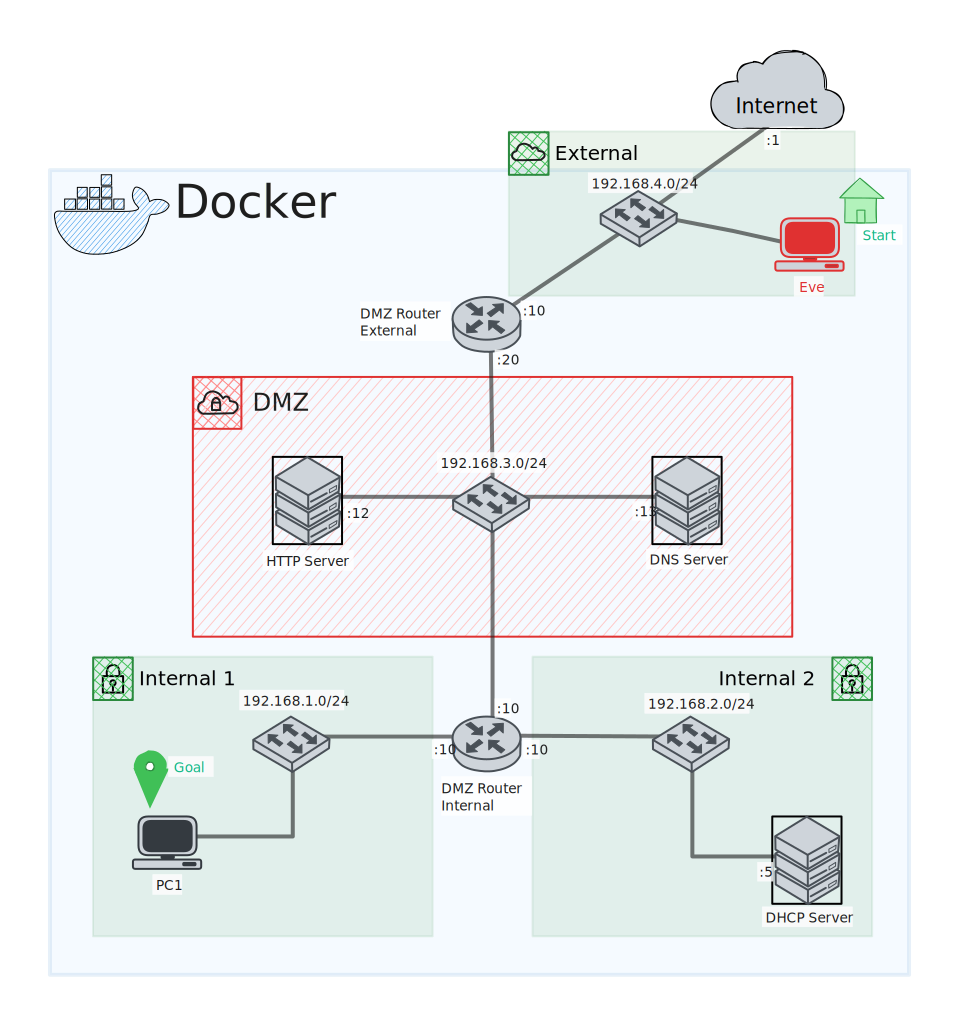
\includegraphics[width=\textwidth]{images/Diagram1.png}
    \caption{Detailed Architecture of our project's network}
    \label{fig:2}
\end{figure}
\newpage

\subsection{Appendix 2 : GANTT Diagram}
\label{Appendix2}
\begin{figure}[bp!]
    \centering
    \includegraphics[scale = 0.8]{images/gantt_diagram.pdf}
\end{figure}
\newpage


\includepdf[pages=1,pagecommand=\thispagestyle{plain},pagecommand=\subsection{Appendix 3 : Red Teaming Documentation}\label{Appendix3}]{DokuFurPentesting/DokuFurPentesting.pdf}
\includepdf[pages=2-,pagecommand=\thispagestyle{plain}]{DokuFurPentesting/DokuFurPentesting.pdf}
\newpage

\includepdf[pages=1,pagecommand=\thispagestyle{plain},pagecommand=\subsection{Appendix 4 : System Administration Documentation}\label{Appendix4}]{DokuFurSysadmin/DokuFurSysadmin.pdf}
\includepdf[pages=2-,pagecommand=\thispagestyle{plain}]{DokuFurSysadmin/DokuFurSysadmin.pdf}
\newpage
\end{document}
